\section{Hiperbolična geometrija} \label{sec:hipgeom}

Hiperbolična geometrija se od evklidske razlikuje v tem, da aksiom

\begin{aksiom}
    Za poljubno premico \(p\) in točko \(A\), ki ne leži na premici \(p\), obstaja natanko ena premica \(q\), ki vsebuje \(A\) in ne seka premice \(p\).
\end{aksiom}

\noindent nadomestimo z

\begin{aksiom}
    Obstajata premica \(p\) in točka \(A\), ki ne leži na premici \(p\), tako, da obstajata vsaj dve premici \(q\) in \(r\), ki vsebujeta \(A\) in ne sekata premice \(p\).
\end{aksiom}

\noindent Nov aksiom prinaša veliko posledic, med drugim tudi drugo metriko; \emph{hiperbolično metriko}, katere lastnosti bomo uporabili pri dokazu. Metriko najprej definiramo na enotskem disku \(\DD \coloneq \set{z \in \CC : |z| < 1}\) in jo nato razširimo na bolj splošne množice. Za začetek ponovimo nekaj osnovnih pojmov iz kompleksne analize.

Uporabljamo standardne oznake. Kompleksno število \(z \in \CC\) lahko zapišemo kot vsoto \(z = x + i y\) ali v polarnem zapisu \(z = r e^{i \theta} = r (\cos \theta + i \sin \theta)\). Kot, ki ga oklepata abscisa in premica skozi \(0\) in \(z\), označimo z \(\Arg (z) \in (- \pi, \pi]\) ali \(\arg (z) \in [0, 2 \pi)\). Z \(D_{\delta} (z)\) označimo odprt disk s središčem v \(z\) in radijem \(\delta\). Torej je \(\DD \coloneq D_1 (0)\).

% \begin{definicija}
%     Naj bo \(D\) odprta množica v \(\CC\) in \(f \colon D \to \CC\) funkcija. Če obstaja
%     \[f' (a) \coloneq \lim_{z \to a} \frac{f (z) - f (a)}{z - a},\]
%     tedaj število \(f' (a)\) imenujemo odvod funkcije \(f\) v točki \(a\). Če \(f' (a)\) obstaja za vsak \(a \in D\), potem pravimo, da je \(f\) \emph{holomorfna} funkcija na \(D\).
% \end{definicija}

\begin{definicija}
    Neprazni odprti in povezani podmnožici kompleksnih števil pravimo \emph{območje}.
\end{definicija}

\noindent Intuitivno si \emph{enostavno povezano} območje predstavljamo kot tisto območje, ki nima ``lukenj''. Natančno pa ga definiramo definiramo z naslednjim izrekom.

\begin{definicija}[Riemannov upodobitveni izrek]
    Območje \(D \subsetneq \CC\) je \emph{enostavno povezano} natanko tedaj, ko obstaja konformni izomorfizem (bijektivna holomorfna funkcija) \(\phi \colon D \to \DD\).
\end{definicija}

\vspace{0.5cm}
\noindent Pri dokazu izreka \ref{thm:orbits} si bomo pomagali tudi z inverzom eksponentne preslikave. Ker pa je \(e^{z + 2 \pi i} = e^x (\cos (y + 2 \pi) + i \sin (y + 2 \pi)) = e^z\), je eksponentna preslikava periodična (glej sliko \ref{fig:exponential}) in posledično nima inverza.
\begin{figure}
    \centering
    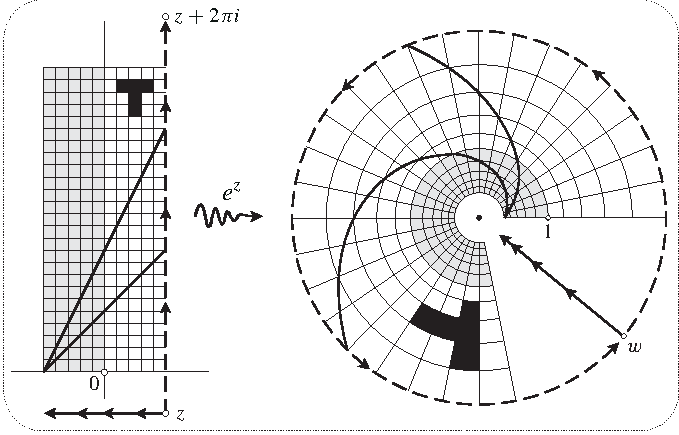
\includegraphics[width=0.6\textwidth]{needham_figure.pdf}
    \caption[Geometrijsko delovanje kompleksne eksponentne preslikave]{Geometrijska vizualizacija kompleksne eksponentne preslikave. Ilustracija je povzeta po knjigi \cite{Needham_1997}}
    \label{fig:exponential}
\end{figure}
Res, naj bo \(w = u + i v\). Rešimo enačbo:
\begin{align*}
    e^w = z &\iff e^u (\cos v + i \sin v) = x + i y\\
            &\iff e^u = \sqrt{x^2 + y^2} \quad \text{in} \quad v = \Arg z + 2 k \pi.
\end{align*}
Torej je \(e^w = z\) natanko tedaj, ko je
\[w = \ln |z| + i \Arg z + 2 k \pi i,\]
za vsak \(k \in \ZZ\). Prav tako bi lahko namesto \(\Arg\) izbrali \(\arg\). Da lahko definiramo inverz, moramo domeno omejiti. Naj bo \(\theta \in \RR\). Potem je
\[\begin{multlined}[10cm]
    \exp \colon  \set{\zeta \in \CC \colon \theta -\pi < \im \zeta < \theta + \pi}\\
    \to \set{\omega \in \CC \colon \Arg \omega \not\equiv \theta - \pi\ (\operatorname{mod}\, 2 \pi)} \eqcolon U
\end{multlined}\]
bijektivna na \(U\) in ima tam holomorfen inverz \(L \colon U \to \CC\):
\[L (\omega) \coloneq \log |\omega| + i \cdot \prt{\theta + \Arg \frac{\omega}{e^{i \theta}}}.\]
Vsaki taki funkciji \(L\) rečemo \emph{veja logaritma}. Če vzamemo \(\theta = 0\) dobimo \emph{glavno} vejo logaritma. Veje logaritma obstajajo tudi na vsakem preprosto povezanem območju, vendar bodo za nas pomembne le zarezane ravnine \(\CC \setminus [0, \infty)\) in diski, ki ne vsebuje izhodišča. Na primer, imejmo disk \(\Delta \subset \CC\), tako da \(0 \notin \Delta\). Naj bo \(\zeta_0 \in \CC\), da je \(e^{\zeta_0} \in \Delta\). Če vzamemo \(\theta = \im \zeta_0\), dobimo holomorfno preslikavo \(L \colon \Delta \to \CC\), za katero velja \(L (e^{\zeta_0}) = \zeta_0\) ter \(e^{L (\omega)} = \omega\) in \(\im \zeta_0 - \pi < \im L (\omega) < \im \zeta_0 + \pi\) za vsak \(\omega \in \Delta\).

\subsection{Hiperbolična metrika na enotskem disku}

Hiperbolično metriko podamo prek \emph{hiperboličnega ločnega elementa}:
\[\dd \rho_{\DD} (z) = \frac{2 |\dd z|}{1 - |z|^2},\]
ki nam pove, da se infinitezimalna sprememba v točki \(z\) v hiperbolični metriki izrazi kot infinitezimalna sprememba v evklidski metriki, pomnožena s t.i.~\emph{gostoto} hiperbolične metrike
\[\rho_{\DD} (z) = \frac{2}{1 - |z|^2}.\]
Iz tega izhaja naslednja definicija.

\begin{definicija}
    Naj bo \(\gamma \colon [a, b] \to \DD\) odsekoma \(C^1\) krivulja. Njena \emph{hiperbolična dolžina} je
    \[l_{\DD} (\gamma) \coloneq \int_{\gamma} \rho_{\DD} (z) \, | \dd z | = \int_{a}^{b} \frac{2 | \gamma' (t) | }{1 - | \gamma (t) |^2} \, \dd t.\]
\end{definicija}

\noindent Končno hiperbolično metriko definiramo kot sledi.

\begin{definicija}
    \emph{Hiperbolična metrika} je preslikava \(d_{\DD} \colon \DD \times \DD \to [0, \infty)\), definirana kot
    \[d_{\DD} (z, w) \coloneq \inf_{\gamma} l_{\DD} (\gamma),\]
    kjer \(\gamma\) teče po vseh odsekoma \(C^1\) krivuljah v \(\DD\), ki povezujejo točki \(z\) in \(w\).
\end{definicija}

\subsection{Hiperbolična metrika na enostavno povezanih območjih}

Definicijo nam iz enotskega diska na enostavno povezana območja prenese naslednji izrek.

\begin{izrek}[Pick] \label{thm:pick}
    Naj bosta \(U, V \subsetneq \CC\) enostavno povezani območji in \(f \colon U \to V\) holomorfna preslikava. Potem na \(U\) obstaja enolično določen hiperbolični ločni element, da velja naslednje.
    \begin{enumerate}
        \item Za vsak \(z \in \DD\) velja \(\rho_{\DD} (z) = \frac{2}{1 - |z|^2}\).
        \item Preslikava \(f\) ne veča \emph{hiperboličnega odvoda}, to je \[\hder{f (z)}{U}{V} \coloneq |f' (z)| \cdot \frac{\rho_V (f (z))}{\rho_U (z)} \leq 1.\]
        \item Enakost \(\hder{f (z)}{U}{V} = 1\) velja natanko tedaj, ko je \(f\) konformni izomorfizem.
        \item Če je \(U \subsetneq V\), potem za vsak \(z \in U\) velja \(\rho_U (z) > \rho_V (z)\). 
    \end{enumerate}
\end{izrek}

\noindent Druga in tretja točka sta pripravni za eksplicitno računanje gostot hiperbolične metrike.

\begin{trditev}[Zgledi hiperbolične metrike] \label{prop:hypexamples} \mbox{}
    \begin{enumerate}
        \item Za desno polravnino \(\HH \coloneq \set{ z \in \CC : \re (z) > 0 }\) je \(\rho_\HH = \frac{1}{\re (z)}\).
        \item Za zgornjo polravnino \(\KK \coloneq \set{z \in \CC : \im (z) > 0}\) je \(\rho_{\KK} (z) = \frac{1}{\im (z)}\)
        \item Za pas \(S \coloneq \set{z \in \CC : |\im (z)| < \pi}\) višine \(2 \pi\) je \(\rho_{S} = \frac{1}{2 \cos (\im (z) / 2)}\).
        \item Za zarezani ravnini velja
            \[
                \rho_{\CC \setminus [0, \infty)} (z) = \frac{1}{2 |z| \sin (\arg (z) / 2)},
                \qquad
                \rho_{\CC \setminus (-\infty, 0]} (z) = \frac{1}{2 |z| \cos (\Arg (z) / 2)}.
            \]
    \end{enumerate}
\end{trditev}

\begin{dokaz}
    Uporabimo izrek \ref{thm:pick} na štirih konformnih izomorfizmih. Naj bo \(\varphi_1 \colon \HH \to \DD\); \(z \mapsto (1 - z) / (1 + z)\). Potem je
    \[\rho_{\HH} (z) = \rho_{\DD} (\varphi_1 (z)) \cdot \abs{\varphi_1' (z)} = \frac{2}{1 - |\varphi_1 (z)|^2} \cdot \frac{2}{|z + 1|^2} = \frac{4}{|1 + z|^2 - |1- z|^2}.\]
    Za \(z = x + i y\) razpišemo \(|1 \pm z|^2 = 1 \pm 2x + x^2 + y^2\) in dobimo želen rezultat. Naj bo \(\varphi_2 (z) \colon \KK \to \DD\); \(\varphi_2 (z) = (z - i) / (z + i)\). Potem po zgornjem postopku dobimo
    \[\rho_{\KK} (z) = \rho_{\DD} (\varphi_2 (z)) \cdot \abs{\varphi_2' (z)} = \frac{4}{|z + i|^2 - |z - i|^2} = \frac{1}{\im (z)}.\]
    Naj bo \(\varphi_3 \colon S \to \HH\); \(z \mapsto e^{z / 2}\). Potem je
    \[\rho_S (z) = \rho_{\HH} (\varphi_2 (z)) \cdot |\varphi_2' (z)| = \frac{|\varphi_2 (z)|}{2 \re \varphi_2 (z)} = \frac{1}{2 \cos (\arg (\varphi_2 (z)))} = \frac{1}{2 \cos (\im (z) / 2)}.\]
    Naj bo \(\varphi_4 \colon \CC \setminus (- \infty, 0] \to \HH\); \(z \mapsto \sqrt{z}\). To je konformni izomorfizem, če se omejimo na rešitev \(r e^{i \theta} \mapsto \sqrt{r} e^{i \theta / 2}\) za \(\theta \in (- \pi, \pi)\). Potem je
    \[\rho_{\CC \setminus (- \infty, 0]} (z) = \rho_{\HH} (\varphi_4 (z)) \cdot |\varphi_4' (z)| = \frac{1}{2 |\sqrt{z}| \re (\sqrt{z})}.\]
    Dobljeno poenostavimo s polarnim zapisom, da dobimo
    \[\frac{1}{2 r \cos (\theta / 2)} = \frac{1}{2 |z| \cos (\Arg (z) / 2)}.\]
    % \[\rho_{\CC \setminus [0, \infty)} (z) = \rho_{\HH} (\varphi_2 (z)) \cdot |\varphi_2' (z)| = \frac{2 |z|}{\re (- z^2)}.\]
    % Uporabimo polarni zapis \(z = r e^{i \theta}\), da dobimo \(- z^2 = - r^2 e^{2 i \theta}\) in \(\re (- r^2 e^{2 i \theta}) = - r^2 \cos (2 \theta)\). Zato z uporabo formule \(\cos (2 \theta) = \cos^2 \theta - \sin^2 \theta\) dobimo
    % \[\frac{2 |z|}{\re (- z^2)} = \frac{2}{- r \cos (2 \theta)} = \frac{2}{r (\sin^2 \theta - \cos^2 \theta)}\]
\end{dokaz}
